
%% bare_conf.tex
%% V1.3
%% 2007/01/11
%% by Michael Shell
%% See:
%% http://www.michaelshell.org/
%% for current contact information.
%%
%% This is a skeleton file demonstrating the use of IEEEtran.cls
%% (requires IEEEtran.cls version 1.7 or later) with an IEEE conference paper.
%%
%% Support sites:
%% http://www.michaelshell.org/tex/ieeetran/
%% http://www.ctan.org/tex-archive/macros/latex/contrib/IEEEtran/
%% and
%% http://www.ieee.org/

%%*************************************************************************
%% Legal Notice:
%% This code is offered as-is without any warranty either expressed or
%% implied; without even the implied warranty of MERCHANTABILITY or
%% FITNESS FOR A PARTICULAR PURPOSE! 
%% User assumes all risk.
%% In no event shall IEEE or any contributor to this code be liable for
%% any damages or losses, including, but not limited to, incidental,
%% consequential, or any other damages, resulting from the use or misuse
%% of any information contained here.
%%
%% All comments are the opinions of their respective authors and are not
%% necessarily endorsed by the IEEE.
%%
%% This work is distributed under the LaTeX Project Public License (LPPL)
%% ( http://www.latex-project.org/ ) version 1.3, and may be freely used,
%% distributed and modified. A copy of the LPPL, version 1.3, is included
%% in the base LaTeX documentation of all distributions of LaTeX released
%% 2003/12/01 or later.
%% Retain all contribution notices and credits.
%% ** Modified files should be clearly indicated as such, including  **
%% ** renaming them and changing author support contact information. **
%%
%% File list of work: IEEEtran.cls, IEEEtran_HOWTO.pdf, bare_adv.tex,
%%                    bare_conf.tex, bare_jrnl.tex, bare_jrnl_compsoc.tex
%%*************************************************************************

% *** Authors should verify (and, if needed, correct) their LaTeX system  ***
% *** with the testflow diagnostic prior to trusting their LaTeX platform ***
% *** with production work. IEEE's font choices can trigger bugs that do  ***
% *** not appear when using other class files.                            ***
% The testflow support page is at:
% http://www.michaelshell.org/tex/testflow/



% Note that the a4paper option is mainly intended so that authors in
% countries using A4 can easily print to A4 and see how their papers will
% look in print - the typesetting of the document will not typically be
% affected with changes in paper size (but the bottom and side margins will).
% Use the testflow package mentioned above to verify correct handling of
% both paper sizes by the user's LaTeX system.
%
% Also note that the "draftcls" or "draftclsnofoot", not "draft", option
% should be used if it is desired that the figures are to be displayed in
% draft mode.
%
\documentclass[conference]{IEEEtran}
% Add the compsoc option for Computer Society conferences.
%
% If IEEEtran.cls has not been installed into the LaTeX system files,
% manually specify the path to it like:
% \documentclass[conference]{../sty/IEEEtran}





% Some very useful LaTeX packages include:
% (uncomment the ones you want to load)


% *** MISC UTILITY PACKAGES ***
%
%\usepackage{ifpdf}
% Heiko Oberdiek's ifpdf.sty is very useful if you need conditional
% compilation based on whether the output is pdf or dvi.
% usage:
% \ifpdf
%   % pdf code
% \else
%   % dvi code
% \fi
% The latest version of ifpdf.sty can be obtained from:
% http://www.ctan.org/tex-archive/macros/latex/contrib/oberdiek/
% Also, note that IEEEtran.cls V1.7 and later provides a builtin
% \ifCLASSINFOpdf conditional that works the same way.
% When switching from latex to pdflatex and vice-versa, the compiler may
% have to be run twice to clear warning/error messages.






% *** CITATION PACKAGES ***
%
%\usepackage{cite}
% cite.sty was written by Donald Arseneau
% V1.6 and later of IEEEtran pre-defines the format of the cite.sty package
% \cite{} output to follow that of IEEE. Loading the cite package will
% result in citation numbers being automatically sorted and properly
% "compressed/ranged". e.g., [1], [9], [2], [7], [5], [6] without using
% cite.sty will become [1], [2], [5]--[7], [9] using cite.sty. cite.sty's
% \cite will automatically add leading space, if needed. Use cite.sty's
% noadjust option (cite.sty V3.8 and later) if you want to turn this off.
% cite.sty is already installed on most LaTeX systems. Be sure and use
% version 4.0 (2003-05-27) and later if using hyperref.sty. cite.sty does
% not currently provide for hyperlinked citations.
% The latest version can be obtained at:
% http://www.ctan.org/tex-archive/macros/latex/contrib/cite/
% The documentation is contained in the cite.sty file itself.






% *** GRAPHICS RELATED PACKAGES ***
%
\usepackage{graphicx}
\ifCLASSINFOpdf
  % \usepackage[pdftex]{graphicx}
  % declare the path(s) where your graphic files are
  % \graphicspath{{../pdf/}{../jpeg/}}
  % and their extensions so you won't have to specify these with
  % every instance of \includegraphics
  % \DeclareGraphicsExtensions{.pdf,.jpeg,.png}
\else
  % or other class option (dvipsone, dvipdf, if not using dvips). graphicx
  % will default to the driver specified in the system graphics.cfg if no
  % driver is specified.
  % \usepackage[dvips]{graphicx}
  % declare the path(s) where your graphic files are
  % \graphicspath{{../eps/}}
  % and their extensions so you won't have to specify these with
  % every instance of \includegraphics
  % \DeclareGraphicsExtensions{.eps}
\fi
% graphicx was written by David Carlisle and Sebastian Rahtz. It is
% required if you want graphics, photos, etc. graphicx.sty is already
% installed on most LaTeX systems. The latest version and documentation can
% be obtained at: 
% http://www.ctan.org/tex-archive/macros/latex/required/graphics/
% Another good source of documentation is "Using Imported Graphics in
% LaTeX2e" by Keith Reckdahl which can be found as epslatex.ps or
% epslatex.pdf at: http://www.ctan.org/tex-archive/info/
%
% latex, and pdflatex in dvi mode, support graphics in encapsulated
% postscript (.eps) format. pdflatex in pdf mode supports graphics
% in .pdf, .jpeg, .png and .mps (metapost) formats. Users should ensure
% that all non-photo figures use a vector format (.eps, .pdf, .mps) and
% not a bitmapped formats (.jpeg, .png). IEEE frowns on bitmapped formats
% which can result in "jaggedy"/blurry rendering of lines and letters as
% well as large increases in file sizes.
%
% You can find documentation about the pdfTeX application at:
% http://www.tug.org/applications/pdftex





% *** MATH PACKAGES ***
%
%\usepackage[cmex10]{amsmath}
% A popular package from the American Mathematical Society that provides
% many useful and powerful commands for dealing with mathematics. If using
% it, be sure to load this package with the cmex10 option to ensure that
% only type 1 fonts will utilized at all point sizes. Without this option,
% it is possible that some math symbols, particularly those within
% footnotes, will be rendered in bitmap form which will result in a
% document that can not be IEEE Xplore compliant!
%
% Also, note that the amsmath package sets \interdisplaylinepenalty to 10000
% thus preventing page breaks from occurring within multiline equations. Use:
%\interdisplaylinepenalty=2500
% after loading amsmath to restore such page breaks as IEEEtran.cls normally
% does. amsmath.sty is already installed on most LaTeX systems. The latest
% version and documentation can be obtained at:
% http://www.ctan.org/tex-archive/macros/latex/required/amslatex/math/





% *** SPECIALIZED LIST PACKAGES ***
%
%\usepackage{algorithmic}
% algorithmic.sty was written by Peter Williams and Rogerio Brito.
% This package provides an algorithmic environment fo describing algorithms.
% You can use the algorithmic environment in-text or within a figure
% environment to provide for a floating algorithm. Do NOT use the algorithm
% floating environment provided by algorithm.sty (by the same authors) or
% algorithm2e.sty (by Christophe Fiorio) as IEEE does not use dedicated
% algorithm float types and packages that provide these will not provide
% correct IEEE style captions. The latest version and documentation of
% algorithmic.sty can be obtained at:
% http://www.ctan.org/tex-archive/macros/latex/contrib/algorithms/
% There is also a support site at:
% http://algorithms.berlios.de/index.html
% Also of interest may be the (relatively newer and more customizable)
% algorithmicx.sty package by Szasz Janos:
% http://www.ctan.org/tex-archive/macros/latex/contrib/algorithmicx/




% *** ALIGNMENT PACKAGES ***
%
%\usepackage{array}
% Frank Mittelbach's and David Carlisle's array.sty patches and improves
% the standard LaTeX2e array and tabular environments to provide better
% appearance and additional user controls. As the default LaTeX2e table
% generation code is lacking to the point of almost being broken with
% respect to the quality of the end results, all users are strongly
% advised to use an enhanced (at the very least that provided by array.sty)
% set of table tools. array.sty is already installed on most systems. The
% latest version and documentation can be obtained at:
% http://www.ctan.org/tex-archive/macros/latex/required/tools/


%\usepackage{mdwmath}
%\usepackage{mdwtab}
% Also highly recommended is Mark Wooding's extremely powerful MDW tools,
% especially mdwmath.sty and mdwtab.sty which are used to format equations
% and tables, respectively. The MDWtools set is already installed on most
% LaTeX systems. The lastest version and documentation is available at:
% http://www.ctan.org/tex-archive/macros/latex/contrib/mdwtools/


% IEEEtran contains the IEEEeqnarray family of commands that can be used to
% generate multiline equations as well as matrices, tables, etc., of high
% quality.


%\usepackage{eqparbox}
% Also of notable interest is Scott Pakin's eqparbox package for creating
% (automatically sized) equal width boxes - aka "natural width parboxes".
% Available at:
% http://www.ctan.org/tex-archive/macros/latex/contrib/eqparbox/





% *** SUBFIGURE PACKAGES ***
%\usepackage[tight,footnotesize]{subfigure}
% subfigure.sty was written by Steven Douglas Cochran. This package makes it
% easy to put subfigures in your figures. e.g., "Figure 1a and 1b". For IEEE
% work, it is a good idea to load it with the tight package option to reduce
% the amount of white space around the subfigures. subfigure.sty is already
% installed on most LaTeX systems. The latest version and documentation can
% be obtained at:
% http://www.ctan.org/tex-archive/obsolete/macros/latex/contrib/subfigure/
% subfigure.sty has been superceeded by subfig.sty.



%\usepackage[caption=false]{caption}
%\usepackage[font=footnotesize]{subfig}
% subfig.sty, also written by Steven Douglas Cochran, is the modern
% replacement for subfigure.sty. However, subfig.sty requires and
% automatically loads Axel Sommerfeldt's caption.sty which will override
% IEEEtran.cls handling of captions and this will result in nonIEEE style
% figure/table captions. To prevent this problem, be sure and preload
% caption.sty with its "caption=false" package option. This is will preserve
% IEEEtran.cls handing of captions. Version 1.3 (2005/06/28) and later 
% (recommended due to many improvements over 1.2) of subfig.sty supports
% the caption=false option directly:
%\usepackage[caption=false,font=footnotesize]{subfig}
%
% The latest version and documentation can be obtained at:
% http://www.ctan.org/tex-archive/macros/latex/contrib/subfig/
% The latest version and documentation of caption.sty can be obtained at:
% http://www.ctan.org/tex-archive/macros/latex/contrib/caption/




% *** FLOAT PACKAGES ***
%
%\usepackage{fixltx2e}
% fixltx2e, the successor to the earlier fix2col.sty, was written by
% Frank Mittelbach and David Carlisle. This package corrects a few problems
% in the LaTeX2e kernel, the most notable of which is that in current
% LaTeX2e releases, the ordering of single and double column floats is not
% guaranteed to be preserved. Thus, an unpatched LaTeX2e can allow a
% single column figure to be placed prior to an earlier double column
% figure. The latest version and documentation can be found at:
% http://www.ctan.org/tex-archive/macros/latex/base/



%\usepackage{stfloats}
% stfloats.sty was written by Sigitas Tolusis. This package gives LaTeX2e
% the ability to do double column floats at the bottom of the page as well
% as the top. (e.g., "\begin{figure*}[!b]" is not normally possible in
% LaTeX2e). It also provides a command:
%\fnbelowfloat
% to enable the placement of footnotes below bottom floats (the standard
% LaTeX2e kernel puts them above bottom floats). This is an invasive package
% which rewrites many portions of the LaTeX2e float routines. It may not work
% with other packages that modify the LaTeX2e float routines. The latest
% version and documentation can be obtained at:
% http://www.ctan.org/tex-archive/macros/latex/contrib/sttools/
% Documentation is contained in the stfloats.sty comments as well as in the
% presfull.pdf file. Do not use the stfloats baselinefloat ability as IEEE
% does not allow \baselineskip to stretch. Authors submitting work to the
% IEEE should note that IEEE rarely uses double column equations and
% that authors should try to avoid such use. Do not be tempted to use the
% cuted.sty or midfloat.sty packages (also by Sigitas Tolusis) as IEEE does
% not format its papers in such ways.





% *** PDF, URL AND HYPERLINK PACKAGES ***
%
%\usepackage{url}
% url.sty was written by Donald Arseneau. It provides better support for
% handling and breaking URLs. url.sty is already installed on most LaTeX
% systems. The latest version can be obtained at:
% http://www.ctan.org/tex-archive/macros/latex/contrib/misc/
% Read the url.sty source comments for usage information. Basically,
% \url{my_url_here}.





% *** Do not adjust lengths that control margins, column widths, etc. ***
% *** Do not use packages that alter fonts (such as pslatex).         ***
% There should be no need to do such things with IEEEtran.cls V1.6 and later.
% (Unless specifically asked to do so by the journal or conference you plan
% to submit to, of course. )


% correct bad hyphenation here
\hyphenation{op-tical net-works semi-conduc-tor}


\begin{document}
%
% paper title
% can use linebreaks \\ within to get better formatting as desired
%\title{Comparative study of two techniques for clustering in Multi-Hop Wireless Sensor Networks}
\title{Behavioral Correlation: A new approach for clustering sensors in Wireless Sensor Networks}

% author names and affiliations
% use a multiple column layout for up to three different
% affiliations
\author{\IEEEauthorblockN{Fernando Rodrigues}
\IEEEauthorblockA{University of Fortaleza\\Fortaleza - Ceara - Brazil\\
fernandorodrigues@edu.unifor.br}
\and
\IEEEauthorblockN{Angelo Brayner}
\IEEEauthorblockA{University of Fortaleza\\
Fortaleza - Ceara - Brazil\\
brayner@unifor.br}
\and
\IEEEauthorblockN{Jose E. Bessa Maia}
\IEEEauthorblockA{State University of Ceara\\
Fortaleza - Ceara - Brazil\\
jose.maia@uece.br}}

% conference papers do not typically use \thanks and this command
% is locked out in conference mode. If really needed, such as for
% the acknowledgment of grants, issue a \IEEEoverridecommandlockouts
% after \documentclass

% for over three affiliations, or if they all won't fit within the width
% of the page, use this alternative format:
% 
%\author{\IEEEauthorblockN{Michael Shell\IEEEauthorrefmark{1},
%Homer Simpson\IEEEauthorrefmark{2},
%James Kirk\IEEEauthorrefmark{3}, 
%Montgomery Scott\IEEEauthorrefmark{3} and
%Eldon Tyrell\IEEEauthorrefmark{4}}
%\IEEEauthorblockA{\IEEEauthorrefmark{1}School of Electrical and Computer Engineering\\
%Georgia Institute of Technology,
%Atlanta, Georgia 30332--0250\\ Email: see http://www.michaelshell.org/contact.html}
%\IEEEauthorblockA{\IEEEauthorrefmark{2}Twentieth Century Fox, Springfield, USA\\
%Email: homer@thesimpsons.com}
%\IEEEauthorblockA{\IEEEauthorrefmark{3}Starfleet Academy, San Francisco, California 96678-2391\\
%Telephone: (800) 555--1212, Fax: (888) 555--1212}
%\IEEEauthorblockA{\IEEEauthorrefmark{4}Tyrell Inc., 123 Replicant Street, Los Angeles, California 90210--4321}}




% use for special paper notices
%\IEEEspecialpapernotice{(Invited Paper)}




% make the title area
\maketitle


\begin{abstract}
%\boldmath
% Sensor clustering is an efficient strategy to reduce the number of messages
% transmitted to the sink in a multi-hop wireless sensor network. In this work we
% make a comparative study of two sensor clustering techniques: cluster heads and
% representative nodes. These techniques are compared with each other and also
% about the effects on them of incorporating mechanisms of temporal and
% spatial-temporal correlations.

Sensor clustering is an efficient strategy to reduce the number of messages
transmitted to the sink in a multi-hop wireless sensor network. In this work we
present a new approach to clustering based on the behavior exhibited by the
historical data read from sensors. Such approach do not use the existing
spatial distance between the sensors (traditional Spatial Correlation) for
clustering, so that the clusters are formed based %solely 
on the dissimilarity measures from the network sensor nodes.
Furthermore, two scheduling intra-clustering methods are tested: Cluster Heads and
Representative Nodes. These techniques are compared with each other and also
about the effects on them of incorporating mechanisms of temporal and
behavioral correlations, creating the new behavio-temporal correlation.
\end{abstract}
% IEEEtran.cls defaults to using nonbold math in the Abstract.
% This preserves the distinction between vectors and scalars. However,
% if the conference you are submitting to favors bold math in the abstract,
% then you can use LaTeX's standard command \boldmath at the very start
% of the abstract to achieve this. Many IEEE journals/conferences frown on
% math in the abstract anyway.

% no keywords




% For peer review papers, you can put extra information on the cover
% page as needed:
% \ifCLASSOPTIONpeerreview
% \begin{center} \bfseries EDICS Category: 3-BBND \end{center}
% \fi
%
% For peerreview papers, this IEEEtran command inserts a page break and
% creates the second title. It will be ignored for other modes.
\IEEEpeerreviewmaketitle



\section{Introduction}
% no \IEEEPARstart

In continuous environmental monitoring applications the sensors in a dense WSN
generate a data stream that must be transmitted to a Sink to be processed and
stored in a Fusion and Decision Center (FDC). It is widely noted [x, x, x] that
this data stream exhibits strong spatio-temporal correlation.

Consider, for example, a dense WSN used in the monitoring of forest fires in
which a magnitude of temperature is monitored. Suppose further the situation in
which the monitored region is affected by dozens of small forest fires (Figure
1a). A possible graph of the temperature contours lines (level curves) for this
hypothetical situation is presented in Figure 1b. In this case the contours
lines form dozens closed areas resulting in natural groupings in the data.
Moreover, it is very likely that the temperature sensors measurements in dozens
of spatially separated clusters also exhibit high correlation. Insight in
Behavioral Correlation Clustering (BCC) is to group all these small clusters
spatially separated in a single cluster, as opposed to existing spatio-temporal
correlation techniques that would keep as dozens of separate clusters.

BCC is to join in a group the sensors for which the forecasting models for
measurement time series are approximately the same independent of their spatial
proximity.  Note that the BCC naturally captures the spatial grouping, if it
exists, since the correlation is between the sensor time series. Several
measures of similarity, dissimilarity or statistical correlation can be used to
group the sensors based on the its time series. Also, several strategies can be
used to trigger the evaluation of clustering: periodic, sliding windows,
triggering threshold and others.

Note that behavioral correlation clustering (BCC) is enabled by centralized
clustering, being more difficult to implement in distributed correlation or
clustering approaches, among other things, due to the limited range of sensor
transmissions.

\begin{figure}[!htb]
\centering
	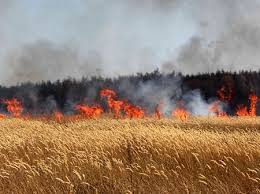
\includegraphics[scale=0.7]{I1.png}
    \caption{Forest fire photography}
    \label{lab}
\end{figure}

\begin{figure}[!htb]
\centering
	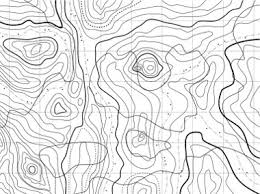
\includegraphics[scale=0.7]{I2.png}
    \caption{Contours lines of temperature}
    \label{lab}
\end{figure}

Sensors are devices used to collect data from the environment related to the
detection or measurement of physical phenomena. Sensors are limited in power,
computational capacity, and memory. Advances in wireless communication have
enabled the development of massive-scale wireless sensor networks (WSN). In a
WSN, sensors are usually scattered in the network and use low-power
communication channels. Thus, sensors disseminate collected data to a base
station, from where the information (query) was originally requested. Wireless
sensor networks (WSNs) have been widely used for environmental monitoring (e.g.,
traffic, habitat), industrial sensing and diagnostics (e.g., factory, supply
chains), infrastructure protection (e.g., water distribution), battlefield
awareness (e.g., multi-target tracking) and context-aware computing (e.g.,
intelligent home) applications.

% Wireless sensor networks (WSNs) has been widely used for capturing environmental
% phenomena data in applications such as study and preservation of ecosystems,
% forest fire alert-and-response and even to study certain species of trees
% \cite{Tolle2005}. However the technological advancement in the technologies for
% construction and communication between sensors, a critical key point is still
% the energy consumption of the nodes, whose highest percentage of consumption
% occurs due to the transmission and reception of data between sensors
% \cite{Yick2008}. Higher accuracy comes at a higher energy cost in many systems.
% 
% To the best of our knowledge, ecological and real sensor data (physical
% environments) is usually strongly correlated \cite{Yoon2005}, so it is easier to
% infer the state of a sensor (from its past and its proximity) \cite{Chu2006}.

WSNs can be categorized into three types, depending on the application or the
use pattern of the network. Thus, there exist WSNs for: {\it (i)} responding to
user queries \cite{Brayner2007}; {\it (ii)} continuously sensing (stream), or;
{\it (iii)} monitoring of certain sporadic events \cite{Ren2007}. These uses are
not mutually exclusive, i.e. in a WSN that responds to queries, one can submit
queries to request data to be sensed with a certain frequency (continuous
sensing) and even data whenever certain events occur. The case that stands out
as being the most critical usage is exactly the continuous sensing, because, in
this case, every certain time interval programmed, the sensor nodes need to take
readings and send the values read through the network, passing from node to
node, until these data reach the sink \cite{Villas2012}.

% WSNs can be categorized into three types, depending on the application or the
% use pattern of the network. They can be used for i) respond to queries, ii)
% continuous sensing (stream) or iii) monitoring of certain sporadic events
% \cite{Ren2007}; however, these uses are not mutually exclusive, i.e. in a WSN
% that responds to queries, we can make queries that request data to be sensed
% with a certain frequency (continuous sensing) and even if alarms are raised when
% certain events occur. The case that stands out as being the most critical usage
% is exactly the continuous sensing, because, in this case, every certain time
% interval programmed, the sensor nodes need to take readings and send the values
% read through the network, passing from node to node, until these data reach the
% sink \cite{Villas2012}.

In spite of advances in WSN technology, a critical key point is still the
energy consumption of sensor nodes. It is well known that communication among
sensors is the activity responsible for the bulk of the power consumption. By
reducing communication costs, energy may be drastically saved, consequently
increasing the WSN's lifetime. An effective strategy to reduce energy
consumption is thus to reduce the number of messages (sensed data) sent across
the network. Nevertheless, the less the number of sensed data is transmitted,
the lower the accuracy of results provided by a WSN is. Thus higher accuracy in
WSNs comes at a higher energy cost.

By now, it is well-known that data collected by WSN are strongly temporally
and/or spatial correlated \cite{Yoon2005, Chu2006}. The traditional spatial data
correlation is related to the idea that the physical proximity among sensors
leads to similar measurements (values) of sensed data, phenomenon known as
"principle of spatial locality". Thus, one can infer that from the capture of
some sensors readings (located in some regions of sensing space), it is possible
to obtain, approximately, the values of the readings of other sensors in its
surroundings. On the other hand, the temporal correlation indicates  the various
readings of a sensor within a time interval have a certain approximation of
their values (principle of temporal locality). such a feature makes possible to
predict (with a certain margin of error) sensed values in the future based on
data collected in the past.

% One of the ways to reduce the energy consumption of sensor nodes and,
% consequently, increase the lifetime of a WSN, is to make the operation of the
% network use the principle of locality of the sensors, that is, the network must
% take into account that the proximity of location of sensors, in general, also
% means an approximation of sensed values \cite{Yick2008}, especially when these
% relate to environmental data. The grouping of sensors in clusters is the main
% technique used to take advantage of the principle of spatial locality in
% reducing the energy consumption of the nodes, because, in this manner, one can
% use only a few representative nodes from each cluster to read the sensed data
% values in a certain region (cluster) in which sensors are spatially correlated.
% Several works have proposed the use of such a technique, with different
% approaches \cite{Chu2006, Villas2012, Singh2010, Liu2007, Shah2007}. However,
% sometimes, even sensors that are not close physically show similar data reading
% patterns. In such cases, a better alternative would be to use clustering
% based on \textit{Behavioral Correlation}, where the network would be able to
% identify similar patterns of sensor readings even in geographically distant
% nodes.

Grouping sensors in clusters is the main technique used to take advantage of the
principle of spatial locality in reducing the energy consumption in WSNs. This
is because one can use only a few representative nodes from each cluster to
sense data in a given spatial region (cluster) in which sensors are spatially
correlated.
Several works have been proposed in order to use that technique, with different
approaches \cite{Chu2006, Villas2012, Singh2010, Liu2007, Shah2007}.
Nonetheless, in several scenarios sensors, which are not spatially close to each
other, may have similar data reading patterns. In such cases, a better
alternative would be to use clustering based on \textit{Behavioral Correlation},
where the network would be able to identify similar patterns of sensor readings
even in geographically distant nodes.

In this paper, we present new approach for clustering sensors in WSNs. The main
features of the proposed approach are: {\it (i)} Cluster formation based on the
\textit{Behavioral Correlation} of the sensors, which, in turn, is computed 
from the time series of sensor readings by applying a \textit{Dissimilarity
Measure}, and; {\it (ii)} the use of a linear regression model for the temporal
suppression of sensed data through the maximum error level (threshold) desired
by the user used to control the data to be sent to the sink. Furthermore, two
different approaches to select of active nodes (scheduling) in each cluster have
been implemented: Representative Nodes (RNs) and Cluster Heads (CHs).

% Another way to reduce the energy consumption of a sensor network, thereby
% increasing the its lifetime, is using the principle of temporal locality
% \cite{Brayner2011}.
% In this way, in an external environment, without artificial interventions, most
% of the time, one can predict the values to be measured by the sensors with a
% certain margin of error from a history of readings and with the application of a
% regression model
%  \footnote{Several studies have proposed the use of this
% technique, taking advantage of predictions across both time and space, with
% different approaches.} (e.g.: linear, like $\bar{S}(t) = A + B(t)$).

% Furthermore, two different approaches to the way of selection of active nodes
% (scheduling) in each cluster were implemented: Representative Nodes (RNs) and
% Cluster Heads (CHs).

The remainder of this document is organized as follows. [To be described\ldots]

Hereafter, we will examine some related works.

\section{Related Work}

In \cite{Vuran2004}, give M representative nodes to send data from the
whole set of N sensors (where $M < N$), based on criteria of calculation of a
Distortion function ($D(M)$) between the sensed values using a threshold
(\textit{distortion bound}) of maximum allowed distortion ($D_{max}$).
The spatial distance between the nodes (representative) directly influences the
calculation of the distortion function through the value of the correlation
coefficient between the values sensed by each node.
The $D(M)$ shows the relationship between the number of M nodes contained in a
region with N nodes ($M < N$) and the correlation coefficients between the node
$n_i$ and $n_j$ and the source event S and the node $n_i$.
That work does not take into account the energy capacity of each node as a
criterion for choosing the representative nodes, although this is a very
important factor due to the restrictive characteristics regarding the energy
consumption of the nodes in a WSN.

In EAST \cite{Villas2012}, sensors are grouped into two levels, under a spatial
correlation approach, while the leader and the representative nodes perform a
temporal suppression technique.
The leader node generates a representative value for each cluster based on data
received by the representative nodes, which form a subset of all the nodes that
sense the same event. The sensed area is divided into "event areas", which in
turn are divided into "correlation regions (c) or cells", where the formers will
be managed, each one, for a "Coordinator node" and the "correlation areas" will
be represented, one by one, by a "Representative node" because a single reading
within this region is enough to represent it.
The size of the correlation region (c) can be decremented or incremented by the
sink according to the application and the characteristics of the event, to
maintain the accuracy of the data collected.

Another way to group sensor nodes into clusters is through measures of
dissimilarity.
In EEDC \cite{Liu2007}, such measures of dissimilarity are calculated by the
sink node for all pairs of nodes of the network, regardless of their location.
The measure of dissimilarity between two nodes is calculated based on up to $3$
parameters, namely:
the differences in magnitude (\textit{M}) and trend (\textit{T}) of the data
values and the geographical/euclidean distance between nodes ($g_{max}dist$).
The criterion of formation of clusters is based on the maximum threshold of
dissimilarity (max\_dst) defined by a tuple (\textit{M}, \textit{T},
$g_{max}dist$), based on the measure of dissimilarity between the nodes. It
works as follows: $1)$ Initially, the data sensed by each node are sent in the
form of a temporal series for the sink. $2)$ The sink then stores all the data
from the sensors and then calculates the measure of dissimilarity (previously
mentioned) for each pair of nodes of the network. $3)$ With the measures
calculated and the maximum threshold of dissimilarity (max\_dst), the sink
divides the nodes into clusters. The sink monitors large variations within a
cluster and dynamically adjusts the cluster in response to the changes in
spatial correlation.
The sink node recalculates the dissimilarity of active sensor nodes (pair to
pair) within each group, at the end of each time interval (time slot), after
having collected the latest samples of each active sensor node. The current
cluster must be divided if the sink node verify that there is at least one
active sensor node reporting significantly different data (i.e. outside the
max\_dst threshold with other nodes in the same cluster).
For computational reasons, it always takes into account the maximum distance
between the sensors in the calculation of dissimilarity measures.
That work does not takes into account the energy reserve of each node as a
criterion for choosing representative nodes (it is used an algorithm that makes,
simultaneously, the equitable scheduling - round robin - along with the random
choice of representatives nodes).
Furthermore, the proposal does not deal with the partial reassembly (formation
of new clusters from the union of other existing ones) of the nodes that have a
low dissimilarity (i.e. high similarity), since this measure could result in a
greater energy saving for the nodes of the network.

The spatial correlation through the formation of clusters is addressed in
\cite{Pham2010} in the form a flooding algorithm where the sink node starts to
send messages to the other nodes of the network, inviting them to form groups
from criteria such as a dissimilarity measure, in addition to the physical
proximity between nodes, since, of course, the message forwarding in a WSN
occurs between adjacent nodes (i.e. geographically close). Cluster Heads (CHs)
are selected, basically, by 2 parameters: {\it (i)} the nodes that are one hop
from the ancestor that sent the message calculate the measure of dissimilarity
with the mean value informed in the message and then those that are within the
threshold of dissimilarity if they apply for CH, where {\it (ii)} it is said to
be the CH the one that have higher level of energy reserve.
We should notice that, during the process of forming clusters, the nodes that
will form the communication backbone between each Cluster Head node and the sink
are also configured. A scheduling of each cluster is done through round robin in
order to decide which member node that will be active in each time slot making
the sensing and sending the data to its respective CH.
Each cluster has a CH and a Gateway (GW), which connects that cluster to the
neighbor cluster (or with the sink node), in the first case through a Cluster
Extend (EC or EXT).
Additionally, each cluster can obviously have several members (MEM) and also
several EC's.
The process of cluster split (formation of new clusters) is delegated to the GW
(Gateway) of each cluster, and not the CH or the sink, which do not need to be
activated for such a task. The weak point is the process of forming clusters, in
which there is an intensive exchange of messages, scattering a significant
amount of energy from the network sensors, in addition to the process of
regrouping of nodes (merge) into new unified clusters, which is only fired by
the sink using a global approach, i.e. to the entire network, not being
predicted, thus, partial regrouping of the clusters.

In \cite{Shah2007}, the spatial correlation is explored by a mechanism called
the GSC (Gridiron Spatial Correlation), where the sensed region has a Cluster
Head that will be in the center of the region delimited by r (radius of the
monitored region), which will be divided into correlated regular regions
(quadratic), according to the spatial density level chosen, defined through
$\theta$ (size of the correlation region equal to $\theta^2$). In this way,
active sensors will be chosen according to 2 basic parameters: {\it (i)} the
proximity of the them regarding the center of the regions correlated and {\it
(ii)} their energy level must be within a certain threshold, above the ones of
their closest neighbours. The scheduling of active nodes works through the
passage of a list by the cluster-head for all nodes (active and inactive, the
latter being momentarily enabled only to receive the list) with the nodes being
active in each time slot, where this configuration is only changed when one of
the active nodes has its energy level below the threshold established. Although
this solution considers the energy level of the nodes in the choice of the
representative nodes (active), and the article mentions that the sizes of the
rectangles can be reconfigured, and that they are considered independent of each
other, that work does not describe how the the energy threshold is calculated
neither how this reconfiguration of the sizes of the rectangles are done and not
even gives examples of the that.

In \cite{Chu2006}, the authors propose the use of probabilistic models
distributed among the sensor nodes of the network, which would consider the
spatial and temporal correlations between the readings of all nodes of the
network, through the use of a probability distribution function (PDF) and a
transition model, in such a way that only the minimum set of data required would
be sent to sink so that the values predicted by such a model do not extrapolate
the maximum error boundary predicted. The advantage of this approach is the
possibility that the probabilistic models jointly represent several different
reading parameters (attributes), such as, temperature, humidity, luminosity,
etc. On the other hand, sensor nodes may need to communicate with each other to
spatially correlate the data, which brings an energetic cost of intra-sensors
communication. In addition, most of the general computation made by the system
is executed by the sensors (source), bringing even more energy expenditure for
them. In this way, such approach becomes inappropriate for sensor networks.

%\section{Proposed Approach}
\section{Implementing Behavioral Correlation in WSNs}

Our approach, called \textit{BTCWSN} - Behavio-Temporal Correlation in Wireless
Sensor Networks, uses two simple principles:
{\it (i)} Cluster formation (or clustering) based on the \textit{behavioral
correlation} of the sensors (optionally using also spatial correlation),
obtained from the time series of sensor readings with use of
\textit{Dissimilarity Measure} \cite{Liu2007}, whence representative nodes are
chosen, reduce sending data over the network, and {\it (ii)} Using a linear
regression model for the temporal suppression of sending data (calculation of
the regression equation coefficients) through the maximum error level
(threshold) desired by the user used to control the data to be sent to the sink.

The traditional Spatial Correlation is related to the idea that the physical
proximity between sensors leads the approximate measurements (values) sensed data for
these sensors, i.e. the values read by such sensors also have a certain margin
of difference between their values, which is known as "principle of spatial
locality". That is, one can infer that from the capture of some sensors readings
(located in some regions of sensing space), it is possible to obtain, roughly,
the values of the readings of other sensors in its surroundings.
Our method exploits \textit{Dissimilarity Measure} \cite{Liu2007} in order to
cluster the sensors by \textit{behavioral correlation}, which takes into account
the correlation between the historical values of the sensors and not only the
spatial proximity of the sensors (optional).

On the other hand, the Temporal Correlation still exists, such that the various
readings that a sensor performs within a certain time interval, also exhibit a
certain approximation of their values, what is known as "principle of temporal
locality". In this way, it is possible predict (with a certain margin of
error) sensed values through the use of an equation of regression, reducing the
number of required readings during a time interval. When together the two
concepts described above, we obtain the basic principle used in our algorithm,
called "Behavio-Temporal Correlation".

The functioning of the algorithm is based on two principles: {\it (i)} formation
of clusters from the correlation of behavioral data (optionally using spatial
correlation), obtained from the time series of readings of the sensors and the
use of \textit{Dissimilarity Measures}, providing that representative nodes
reduce sending data over the network and {\it (ii)} using a linear regression
model for temporal suppression of sending data (calculation of the coefficients
of the regression equation), through the maximum error level (threshold) desired
by the user used to control the data being sent to the sink.

In addition, two different approaches for scheduling intra-cluster were
implemented. In the first one, called Representative Nodes (RNs), only one node
in each cluster is chosen at each time (by the sink node) to represent that
cluster, making data sensing and predictions. In the second method, called
Cluster Heads (CHs), on the other hand, one sensor node (the CH) in each cluster
is selected to manage the data readings that are made by all other nodes in
cluster.

\subsection{Description of Energy consumption reduction algorithm of sensors using 
Behavio-Temporal Correlation (BTCWSN):}

Initially, the network needs to be configured from the setting of its working
parameters. To this end, it is necessary to specify:

\begin{itemize}
  \item The size of the initial slot time, i.e. the amount of cycles that each
sensor must monitor/send to the sink initially;
  \item The type of data to be sensing. For example: 't' for "temperature",
'h' for "humidity", 'l' for ``luminosity'' or 'v' for "voltage";
  \item The threshold of acceptable temporal error (percentage) for the
determination of us sensors, which can be between 0.0 (does not accept mistakes)
and 1.0 (accepts any error);
  \item The threshold of acceptable magnitude difference (Spatial error) for the
determination of sensors nodes;
  \item The maximum distance acceptable for the formation of clusters, that is,
the greatest distance possible between two sensors so that they are classified
as belonging to the same cluster. If this is equal to zero (0.0), such a
distance limit will not be considered (\textit{behavioral correlation});
  \item The type of cluster sensing configuration to be chosen, which may be of
the type:
	\begin{enumerate}
	  	\item Representative Nodes (RN), where only these knots (one per cluster)
	  	will be sensing while the others are in a "spleep state"; and
		\item Cluster Heads (CH), where all nodes in the cluster are sensing
		(including own CH) and send the data to the CH, which in turn concentrates the
		information before send them to the sink;
	\end{enumerate}
  \item The minimum occupancy rate per cluster, i.e. the average number of
sensors per cluster on the network, which is used to fire the merge (regrouping)
process;
  \item The maximum number of acceptable "novelties per sensor" (NPS), i.e. the
maximum amount prediction errors that do not generate recalculation messaging
of the coefficients of Regression Equation for a given sensor node (be it a
representative node or an any node/Cluster Head);
  \item Only for the case of the use of Cluster Heads, the maximum number of
acceptable "novelties by cluster" (NPC), that is, the maximum amount of
prediction error messages received by their respective CH (sent by the
respective sensors cluster nodes) that do not generate message submission
(recalculation of the coefficients of the regression equation) of CH for sink.
\end{itemize}

Some parameters, however, are automatically configured by the algorithm, such as
example:

\begin{itemize}
  \item The maximum number of predictions/readings that each representative
sensor node must perform even the choice of a new representative node for that
cluster. This parameter is configured /calculated in a manner inversely
proportional to the size of the cluster in question (i.e. the number of sensor
nodes that belong to the same cluster) for reasons of energy balance from 
nodes within a same cluster;  
\end{itemize}

The algorithm can be divided into nine steps given below:

\begin{enumerate}
  \item Initial Readings: Set of readings (rounds) to be performed to load the
initial data into the sink before it can combine sensors into clusters, set the
Representative Nodes or Cluster Heads and calculate the coefficients of the
regression equation.
  \item Clustering Sensor Nodes - Behavioral Correlation: After the sink get the
baseline data (initial readings), the next step is to analyze such data (time
series) sent by all sensor nodes to classify them into Clusters of accordance
with the \textit{Dissimilarity Measures} (DM) read data passed. The DM is based
on 2 (or 3) criteria\footnote{Depending of the kind of \textit{behavioral
correlation} desired: with Spatial Correlation or without Spatial Correlation}
to decide if two sensors are in a same cluster or not.
  \item Determination of Representative Nodes / Cluster Heads: Once the sensors
are classified in clusters, the Representative Nodes or Cluster Heads of each
cluster will be chosen through 2 criteria, applied to all nodes of each sensor
clusters:

  \begin{enumerate}
    \item the sensor with a higher battery energy level
    \item the sensor with the shortest distance (the most
    next in number of hops) from the sink node (in the event of a tie)
  \end{enumerate}

  \item Calculation of the Coefficients of the Regression Equation and the
Maximum Amount of Predictions to be Performed: Once chosen the Representative
Nodes/Cluster Heads of each cluster, the sink must compute the coefficients of
the regression equation. If Representative Nodes are used, must also be
calculated the maximum number of predictions/readings each representative sensor
node must run. Then, the sink must inform these data for the respective
representative sensor nodes.
  \item Sensing Loop: In the case of Representative Node, each (Representative)
Node should start running its predictions by checking the respective thresholds:

  \begin{enumerate}
    \item maximum number of predictions to be performed by the Representative
    Node, and
    \item maximum number of prediction errors that can happen without occurs
    sink notification by this fact
  \end{enumerate}
  
In the case of use of Cluster Heads, all nodes of each cluster should start running
their predictions, noting the following thresholds:

  \begin{enumerate}
    \item maximum number of prediction errors that can happen without occurs the
    notification of respective Cluster Head for that fact, and
    \item maximum number of prediction error notifications that can happen without occur
    the sink notification by part of the Cluster Head due to this fact
  \end{enumerate}

  \item Report of "novelties": If the maximum number of prediction errors
allowed is exceeded, the representative sensor node (or the Cluster Head) shall
report such fact by sending message for the sink node, which must choose one of
the two following actions:
  
  \begin{enumerate}
    \item Recalculate the coefficients of the regression equation that
representative node, using the new reading values submitted, or
    \item Choose a new representative node, based on the selection criteria of
representative nodes presented above.
  \end{enumerate} 

  \item Battery level update of Representative Nodes (RNs) in sink: Whenever a
sensor node (representative node or cluster head) send a message to sink, this
should contain the battery level (current) in the sender, in such a way that the
sink can use this information to re-sort such sensors for that with
higher energy level is chosen as Representative Node/Cluster Head of the
cluster.
  
  \item Cluster split process: When the sink check that variations in the
measurements of sensors of a same cluster are above a certain threshold, it must
raise an process of division (split) of such a cluster so that the old one form
(2 or more) new clusters, whose measurements of the sensors are within the limit
of spatial error allowed.
  
  \item Restructuring (merge) clusters: When the number of (divisions of)
clusters achieve a certain ceiling estimated, then the sink should fire a global
process of clusters restructuring, with possible groupings (merge) from
sensors in old different clusters into new clusters.
  
\end{enumerate}

We will then describe each of these steps above, in more detail:  
  
\subsubsection{Initial Readings}

In this step, the sink node (sinkhole) will send a broadcast message (using a
protocol of 'flooding') to all nodes of the network of sensors, which will, in
turn, respond to this message with the requested data, so that the sink can
capture a certain set of 'n' data preliminaries (where 'n' is the size of the
initial timeslot) of all active sensors (containing basically the absolute value
read, the timestamp of the reading, the battery level of the sensor, the round
in the reading and the spatial location of the sensor) which will serve as a
basis for initial formation of the clusters, to be held centrally by the sink.
After the formation of the clusters and choice the representative nodes/cluster
heads, such data will be used as parameters to the calculation of the
coefficients of regression equations of representative nodes or of each of the
nodes of each cluster formed.

\subsubsection{Clustering Sensor Nodes - Behavioral Correlation}

The calculation of \textit{Dissimilarity Measures} between the sensors as
described in \cite{Liu2007}, is accomplished by the sink node, as a criterion
for the formation of clusters, from 2 (or 3) parameters (the third is optional):
the similarity of magnitude (\textit{spacialThresholdError}), the similarity of
trend (\textit{thresholdError}) and the distance (\textit{maxDistance}) between
nodes (in our case, not mandatory). Thus, from the time series of readings of
each sensor, sink performs the comparison of data received through the
calculations of (dis)similarity among all the sensors (peer to peer) as follows:

\begin{enumerate}
    \item If the maximum distance (\textit{maxDistance}) has value greater than
0 (zero) and the spatial distance between the nodes in question is less than
this value, or if the parameter maximum distance (maxDistance) has value equal
to 0 (zero), then go to the next step. Otherwise, the sensors are in different
clusters.
    \item If the average of the differences between the values of the readings
of the sensors is less than or equal to magnitude similarity parameter
(\textit{spacialThresholdError}) and if the percentage similar trends
(growth/decay) of the data of the two sensors is greater or equal to the
parameter of trend similarity (\textit{thresholdError}), so these sensors
will be in the same cluster. Otherwise, they will be in different clusters.
 \end{enumerate}

Thus, at the end of this process, all sensors nodes have been divided /
classified in clusters by the sink, according to initial readings sent / passed
by sensor nodes to the sink and the \textit{Dissimilarity Measures}
parameterized, using the \textit{behavioral correlation} proposed. Whenever the
sink receives a notification of novelties threshold exceeded of a sensor node
(that can be a RN or a CH), it (sink) recalculates the dissimilarity measures
between all nodes of this cluster to check whether it is necessary to perform a
split in such a cluster.

\subsubsection{Determination of Representative Nodes}

From the separation of network sensors in clusters (groups), the sink will hold
two internal ratings in the nodes of each cluster sensors. Such classifications
are described below:

\begin{enumerate}
    \item The nodes are ordered by the criterion of highest energy level (higher
    battery load), largest to smallest
    \item The nodes that have equally the highest energy level, will then be
    classified in according to their distance to the sink, the shortest distance
    to the biggest
 \end{enumerate}

After this classification process, the first one of each cluster node (that is,
the one that has the higher energy level of battery and the shortest distance to
the sink) will be initially chose as Representative Node. This process of
choosing of RNs is repeated for each cluster, whenever a new notification is
received by the sink.

\subsubsection{Calculation of the coefficients of the Regression Equation and
the amount Maximum of Predictions to be performed}

The maximum amount of predictions (reading/prediction loops) for each node
(Representative of each cluster) will be calculated (individually) as being the
starting size time slot divided by amount of nodes in the cluster, namely, will
be inversely proportional to quantity sensor nodes in each cluster. The reason
for this form of calculation is for there to be a better division (fairer) of
energy expenditure between the sensors of the same cluster, causing those
sensors that have similarities in their readings (of a same cluster) to switch
on the monitoring of the area covered by these sensors, increasing the lifetime
total of each cluster and thus contributing to increase the total life time of
the network.
The coefficients calculation of the Regression Equation (A and B) is held by the
sink, for each of the Representative Nodes chosen by using the following
formulas:

$$
A = \bar{S} - B\bar{t}
$$
$$
B = \frac{\sum(t_i-\bar{t})(S_i-\bar{S})}{\sum(t_i-\bar{t})^2}
$$

where
$\bar{S}$ is the average of the sensing values,
$\bar{t}$ is the average of the moment of time at which the sensing was,
$S_i$ is the ith sensing value and 
$t_i$ is the ith moment of sensing time.

After the calculation of the maximum amount of predictions and the coefficients
of the regression equation, the sink sends this data through a message addressed
to the respective Representative Sensor Node, who, in turn, should begin the
process of sensing (reading/prediction).

\subsubsection{Implementation of Sensing Loop}

At this stage, the Representative Node enter into reading / prediction loop, in
such a way that every step, they must verify that the read value (sensing) for
each one is within the bounds of error (threshold) to the value predicted by
calculating the regression equation from / for that node. If the limits of error
are respected, then the Representative Node's regression equation encountered a
hit (hit), otherwise, it must record an error (miss). If the number of errors
(misses) exceeds a certain limit (preset), then such Representative Node must
report the sink, otherwise, the Representative Node must perform such process of
reading/verifying the prediction to the limit the number of predictions made for
that Representative Node by sink, calculated in the previous phase.

\subsubsection{Report of "Novelties"}

During the execution of the sensing loop, when a Representative Node verifies
that the number of errors (misses) exceeded a given threshold (preset), this
node must inform such event to the sink by sending a message, which will contain
still the latest data reads/sensings performed beyond the current level of
sensor battery. When such a message arrives at the sink node, this must update
the data relating the Representative Node (including the battery level) and then
must check one of the following possibilities:

\begin{enumerate}
    \item If there is a need to make a (new) division / split of the cluster,
    with the choice of new Representative Nodes, or
    \item If there is no need of division, but only the choice of a new
    Representative Node for the current cluster, depending on the level of RN
    current battery in relation to other sensor nodes that cluster, or
    \item If there is no need nor of division neither the choice of a new RN,
    simply that the sink perform the calculation of new Coefficients (updated)
    of the regression equation of such a Representative Node, and still retain
    the maximum number of prediction loops that RN (i.e. continuing to counter
    predictions without restarting)
\end{enumerate}

\subsubsection{Battery Level update of Representative Nodes / Cluster Heads}

Whenever a RN / CH send a message to the sink (by reason of the novelties report
or by have reached the maximum number of loops of prediction), this message must
contain the current battery level information (energy reserves) of that node, in
such a way that the sink can update this information and verify the need to
exchange the sensor node to be chosen as RN / CH of the respective cluster.

\subsubsection{Process of Cluster Division (Split)}

This process must be raised by the sink whenever it finds that the set of nodes
sensors grouped in a particular cluster is no longer meeting the minimum
requirements of (dis)similarity required from the initial parameter
configuration data. In this case, the sink must perform the split of the nodes
of a given cluster sensors in two or more new clusters, selecting new
Representative Node (RNs) - one for each of the new clustes - in accordance with
the criteria set out in the "Determination of Representative Nodes". In Addition
to that, the sink must keep a control on the maximum number of divisions
(splits) or the maximum amount of clusters, in such a way that it is capable of
firing the "restructuring process (merge)" cluster to verify this need.

\subsubsection{Cluster Restructuring (Merge)}

Whenever there are a large number of divisions (splits) and the minimum rate
occupation clusters (average of nodes per cluster) on the network
(\textit{minimumOccupancyRatePerCluster}) is disregarded, the sink should fire a
global process of regrouping (merge) or restructuring of the network, such that
all nodes can have their sensors read data reassessed, and thus can be
reconfigured into new clusters that represent better the current state of the
network. Thus, one avoid that, with the passage of time, and consequently, a
increasing number of divisions (splits) of network clusters, can cause the
clusters become smaller, increasing the energy expenditure of the network's
sensors.

% \subsection{BTCWSN-RN - Representative Node Approach}
% 
% \subsection{BTCWSN-CH - Cluster Head Approach}

\section{Data and Experiments}
\label{Data and Experiments}
In our tests, we done a comparative analysis between the following approaches:
1) On approach Naive \cite{Madden2005}, all sensors are network data reads
(sensing) and send immediately these data to the sink; 2) On approach using
Temporal Correlation (Adaga-P*) \cite{Brayner2011}, all nodes are sensors to
read data from the environment, but only those whose readings submit values
outside the margin of error (user-defined threshold) in relation to values
predicted by the use of a regression equation (whose coefficients are calculated
by sink and sent for each sensor), send your data (Novelties) to the sink; 3) On
approach BTCWSN-RN, after the formation of the clusters based on the
\textit{behavioral correlation} proposed, only the Representative Nodes (RNs) of
each cluster perform reading and data (sensing) only those who detect a quantity
of Novelties above the minimum acceptable amount, configured by the user, shall
send such information (novelty) to the sink; 4) in this latter approach,
referred to as BTCWSN-CH, after the clustering (also based on the
\textit{behavioral correlation}), all sensors, including the Cluster Heads (CHs)
choosen, make sensing / prediction, but sending data (Novelties) to the sink is
divided into two phases: At first, only sensors send novelties to their
respective Cluster Head after the occurrence of a minimum threshold of Novelties
(say N) configured by the user; In the second phase, each Cluster Head, in turn,
only relays novelties for sink after receiving a minimum number of notifications
from your sensors (let's say M), also configured by the user.
The approaches 1) and 2) were implemented based on the references. Our proposal
was implemented through the items 3) and 4).
To make the performance evaluation of our work, we use the SinalGo version
v.$0.75.3$ simulator \cite{Sinalgo2007}. The data used for the simulation were
extracted from experiment Intel Lab Data \cite{Intel2004}.

\section{Results and Discussion}

Our tests focused mainly on 3 parameters to evaluate the performance of our
solution (Approaches BTCWSN-RN and BTCWSN-CH, both described in section
\ref{Data and Experiments}) compared to the other two approaches (Naive and
Adaga-P*): 1) The Root Mean Square Error (RMSE) was used to verify the quality
of the values ​​calculated in the sink with the values ​​actually read by the
sensors - the smaller RMSE, better was the approximation in sink of values
​​read by the sensors; 2) The Total Number of Messages sent by all network
sensors, which is an important factor in the energy consumption of the network -
the lower this amount of messages, the greater lifetime of the network, and 3)
The Number of Data Readings (Sensing) performed by all sensor nodes, since this
number is also related to the energy expenditure of sensor nodes, and as the
messages, the lower this number, the more energy durability of the network.

As can be observed in the tables / graphs shown below, at the end of 1000 cycles
execution of the simulation algorithm, the approach 3 (BTCWSN-RN) presented a
RMSE of $0.502$, while we had a number of messages exchanged $96.33\%$ smaller
as well as a number of sensor readings $47.69\%$ lower than the first
approach (Naive). Compared with the approach 2 (Adaga-P*), which showed an
RMSE of $0.467$ (i.e. only $7\%$ less that approach 3), approach 3 had a
number of messages exchanged $12.78\%$ lower and a number of sensor readings
$46.84\%$ lower than the second approach.
With respect to approach 4 (BTCWSN-CH), it presented a RMSE of $0.355$, with a
total number of messages exchanged $97.73\%$ smaller and a number of sensor
readings $20.19\%$ less the first approach (Naive). When compared to approach 2
(Adaga-P*), the approach 4 presented a RMSE $23.98\%$ smaller, with a total
number of messages exchanged $46.01\%$ smaller and a number of sensor readings
$18,90\%$ less.

\begin{table}[h!]
\caption{Evaluation results - Comparison between four approaches (at the end of 1000 cycles)}
\begin{center}
\begin{tabular}{|l||l|l|l|}
\hline
% \multicolumn{6}{|c}{\textbf{1 semestre 2011}}\\
% \hline
Approach (N = 54 sensors) &RMSE &\#Messages &\#Readings \\
\hline\hline
Naive &0 &222242 &52812 \\
\hline
Adaga-P* &0,467 &9340 &51970 \\
\hline
BTCWSN-RN &0,502 &8146 &27626 \\
\hline
BTCWSN-CH &0,355 &5043 &42149 \\
\hline
\end{tabular}
\end{center}
\end{table}

\begin{table}[h!]
\caption{Naive x BTCWSN-RN (Percentage difference at the end of 1000 cycles)}
\begin{center}
\begin{tabular}{|l||l|l|l|}
\hline
% \multicolumn{6}{|c}{\textbf{1 semestre 2011}}\\
% \hline
Approach (N = 54 sensors) &RMSE &\#Messages &\#Readings \\
\hline\hline
Naive (A) &0 &222242 &52812 \\
\hline
BTCWSN-RN (B) &0,502 &8146 &27626 \\
\hline
Diff (A-B) &N/A &$-96,33\%$ &$-47,69\%$ \\
\hline
\end{tabular}
\end{center}
\end{table}

\begin{table}[h!]
\caption{Adaga-P* x BTCWSN-RN (Percentage difference at the end of 1000 cycles)}
\begin{center}
\begin{tabular}{|l||l|l|l|}
\hline
% \multicolumn{6}{|c}{\textbf{1 semestre 2011}}\\
% \hline
Approach (N = 54 sensors) &RMSE &\#Messages &\#Readings \\
\hline\hline
Adaga-P* (A) &0,467 &9340 &51970 \\
\hline
BTCWSN-RN (B) &0,502 &8146 &27626 \\
\hline
Diff (A-B) &$+7,49\%$ &$-12,78\%$ &$-46,84\%$ \\
\hline
\end{tabular}
\end{center}
\end{table}

\begin{table}[h!]
\caption{Naive x BTCWSN-CH (Percentage difference at the end of 1000 cycles)}
\begin{center}
\begin{tabular}{|l||l|l|l|}
\hline
% \multicolumn{6}{|c}{\textbf{1 semestre 2011}}\\
% \hline
Approach (N = 54 sensors) &RMSE &\#Messages &\#Readings \\
\hline\hline
Naive (A) &0 &222242 &52812 \\
\hline
BTCWSN-CH (B) &0,355 &5043 &42149 \\
\hline
Diff (A-B) &N/A &$-97,73\%$ &$-20,19\%$ \\
\hline
\end{tabular}
\end{center}
\end{table}

\begin{table}[h!]
\caption{Adaga-P* x BTCWSN-CH (Percentage difference at the end of 1000 cycles)}
\begin{center}
\begin{tabular}{|l||l|l|l|}
\hline
% \multicolumn{6}{|c}{\textbf{1 semestre 2011}}\\
% \hline
Approach (N = 54 sensors) &RMSE &\#Messages &\#Readings \\
\hline\hline
Adaga-P* (A) &0,467 &9340 &51970 \\
\hline
BTCWSN-CH (B) &0,355 &5043 &42149 \\
\hline
Diff (A-B) &$-23,98\%$ &$-46,01\%$ &$-18,90\%$ \\
\hline
\end{tabular}
\end{center}
\end{table}

% An example of a floating figure using the graphicx package.
% Note that \label must occur AFTER (or within) \caption.
% For figures, \caption should occur after the \includegraphics.
% Note that IEEEtran v1.7 and later has special internal code that
% is designed to preserve the operation of \label within \caption
% even when the captionsoff option is in effect. However, because
% of issues like this, it may be the safest practice to put all your
% \label just after \caption rather than within \caption{}.
%
% Reminder: the "draftcls" or "draftclsnofoot", not "draft", class
% option should be used if it is desired that the figures are to be
% displayed while in draft mode.
%
%\begin{figure}[!t]
%\centering
%\includegraphics[width=2.5in]{myfigure}
% where an .eps filename suffix will be assumed under latex, 
% and a .pdf suffix will be assumed for pdflatex; or what has been declared
% via \DeclareGraphicsExtensions.
%\caption{Simulation Results}
%\label{fig_sim}
%\end{figure}

% Note that IEEE typically puts floats only at the top, even when this
% results in a large percentage of a column being occupied by floats.


% An example of a double column floating figure using two subfigures.
% (The subfig.sty package must be loaded for this to work.)
% The subfigure \label commands are set within each subfloat command, the
% \label for the overall figure must come after \caption.
% \hfil must be used as a separator to get equal spacing.
% The subfigure.sty package works much the same way, except \subfigure is
% used instead of \subfloat.
%
%\begin{figure*}[!t]
%\centerline{\subfloat[Case I]\includegraphics[width=2.5in]{subfigcase1}%
%\label{fig_first_case}}
%\hfil
%\subfloat[Case II]{\includegraphics[width=2.5in]{subfigcase2}%
%\label{fig_second_case}}}
%\caption{Simulation results}
%\label{fig_sim}
%\end{figure*}
%
% Note that often IEEE papers with subfigures do not employ subfigure
% captions (using the optional argument to \subfloat), but instead will
% reference/describe all of them (a), (b), etc., within the main caption.


% An example of a floating table. Note that, for IEEE style tables, the 
% \caption command should come BEFORE the table. Table text will default to
% \footnotesize as IEEE normally uses this smaller font for tables.
% The \label must come after \caption as always.
%
%\begin{table}[!t]
%% increase table row spacing, adjust to taste
%\renewcommand{\arraystretch}{1.3}
% if using array.sty, it might be a good idea to tweak the value of
% \extrarowheight as needed to properly center the text within the cells
%\caption{An Example of a Table}
%\label{table_example}
%\centering
%% Some packages, such as MDW tools, offer better commands for making tables
%% than the plain LaTeX2e tabular which is used here.
%\begin{tabular}{|c||c|}
%\hline
%One & Two\\
%\hline
%Three & Four\\
%\hline
%\end{tabular}
%\end{table}


% Note that IEEE does not put floats in the very first column - or typically
% anywhere on the first page for that matter. Also, in-text middle ("here")
% positioning is not used. Most IEEE journals/conferences use top floats
% exclusively. Note that, LaTeX2e, unlike IEEE journals/conferences, places
% footnotes above bottom floats. This can be corrected via the \fnbelowfloat
% command of the stfloats package.



\section{Conclusion}

As result of our experiments, we show that the use of the \textit{Behavioral
Correlation} approach associated with a temporal correlation technique using two
different methods for intra-cluster scheduling, namely Representative Nodes
(RNs) or Cluster Heads (CHs), brought a great benefit to the energy economy of
Wireless Sensor Networks (WSNs), since, while it remained a low RMS Error for
the data obtained by the sink using such techniques (spacio-temporal
suppression), two important factors in energy expenditure of a sensor network
decrease, which are the total number of messages sent on the network and the
total number of sensor readings.


% conference papers do not normally have an appendix


% use section* for acknowledgement
\section*{Acknowledgment}


The authors would like to thank...





% trigger a \newpage just before the given reference
% number - used to balance the columns on the last page
% adjust value as needed - may need to be readjusted if
% the document is modified later
%\IEEEtriggeratref{8}
% The "triggered" command can be changed if desired:
%\IEEEtriggercmd{\enlargethispage{-5in}}

% references section

% can use a bibliography generated by BibTeX as a .bbl file
% BibTeX documentation can be easily obtained at:
% http://www.ctan.org/tex-archive/biblio/bibtex/contrib/doc/
% The IEEEtran BibTeX style support page is at:
% http://www.michaelshell.org/tex/ieeetran/bibtex/
%\bibliographystyle{IEEEtran}
% argument is your BibTeX string definitions and bibliography database(s)
%\bibliography{IEEEabrv,../bib/paper}
%
% <OR> manually copy in the resultant .bbl file
% set second argument of \begin to the number of references
% (used to reserve space for the reference number labels box)

% \begin{thebibliography}{1}
% 
% \bibitem{IEEEhowto:kopka}
% H.~Kopka and P.~W. Daly, \emph{A Guide to \LaTeX}, 3rd~ed.\hskip 1em plus
%   0.5em minus 0.4em\relax Harlow, England: Addison-Wesley, 1999.
% 
% 
% \end{thebibliography}

%
% The following two commands are all you need in the
% initial runs of your .tex file to
% produce the bibliography for the citations in your paper.
%\bibliographystyle{abbrv}

% \bibliographystyle{unsrt}
% \bibliography{ISCC2014rodrigues_brayner_maia}  % ISCC2014rodrigues_brayner_maia.bib is the name of the Bibliography in this case

\bibliographystyle{IEEEtran}
\bibliography{IEEEabrv,ISCC2014rodrigues_brayner_maia}  % ISCC2014rodrigues_brayner_maia.bib is the name of the Bibliography in this case
% You must have a proper ".bib" file
%  and remember to run:
% latex bibtex latex latex
% to resolve all references




% that's all folks
\end{document}


